\documentclass[12pt]{beamer}
\useoutertheme{infolines}
\useinnertheme{circles}
%\usetheme{rose}
\usecolortheme{seahorse}
\usepackage[T2A]{fontenc}
\usepackage[utf8]{inputenc}
\usepackage[russian, english]{babel}
\usepackage{amssymb}
\usepackage{amsfonts}
\usepackage{textcomp}
\usepackage[all]{xy}
\usepackage{amsthm}
\usepackage{graphicx}
%\usepackage[dvips]{graphicx}
\usepackage{wrapfig}
\usepackage{concrete}
\usepackage{eufrak}
%\usepackage{euler}
\usepackage{babelbib}
\usepackage{multirow}
\usepackage{multicol}
\usepackage{longtable}
\usepackage{cite}
\usepackage{ifthen}
\usepackage{array}
\usepackage{soul}
\usepackage{indentfirst}
\usepackage{varioref}
\usepackage{hyperref}
\usepackage{enumitem}

\title[Иссл-ние работы батарей с LSTM RNN]{Исследование работы батарей с применением Long short-term memory recurrent neyral network}
\author[Лысов А.В., Епрев А.Е.]{Лысов Александр Васильевич\\Епрев Артем Евгеньевич}
\institute[МатМех]{Санкт-Петербургский государственный университет\\ Математико-механический факультет\\Кафедра информатики\\342 группа}
\date{\today}
\begin{document}
\begin{frame}
  \titlepage
\end{frame}
\begin{frame}
  \tableofcontents
\end{frame}
\section{Введение}
\begin{frame}
  \frametitle{Введение}
  \begin{block}{Цель}
  Целью нашей работы является исследование работы батарей.
  \\
  \end{block}
  \begin{block}{Зачем?}
  Литий-ионный батареи используются везде: от наручных часов до электрических автомобилей, поэтому их исследования очень важны.
  \end{block}
\end{frame}
\section{Основная часть}
\subsection{Начальный набор данных}
\begin{frame}
  \frametitle{Исходные данные}
  \begin{block}{}
  Набор данных был взят с сайта ti.arc.nasa.gov и был представлен в расширении .mat.
  \end{block}
  \begin{block}{}
  \begin{itemize}
    \item Набор из четырех литий-ионных батарей (№ 5, 6, 7 и 18) 
    \item 2 цикла:
      \begin{itemize}
        \item Заряд
        \item Разряд
      \end{itemize}
  \end{itemize}
    \end{block}
\end{frame}
\subsection{Обработка данных}
\begin{frame}
  \frametitle{Как можно решить эту проблему?}
  \begin{block}{}

  \end{block}
\end{frame}
\subsection{Идеи методов}
\begin{frame}
  \frametitle{Идеи методов}
  \begin{block}{Наш метод решения данной проблемы состоит из нескольких этапов:}

  \end{block}
\end{frame}
\subsection{Реализация}
\begin{frame}
  \frametitle{Реализация}
  \begin{block}{Язык и библиотеки}
  Программа написана на языке Python 2, и в ней использовались библиотеки keras, sklearn, numpy, pandas, matplotlib, os, scipy.
  \end{block}
\end{frame}
\begin{frame}
  \begin{block}{Загрузка данных}
    При помощи метода loadmat из scipy.io был загружен изначальный набор данных циклов батарей. Структура была неудобна для дальнейшего использования, а именно, имела вид: \\
      \begin{displaymath}
      dataset[fileName][0, 0][0][0][i][3][0][0][k][0][j],
      \end{displaymath}
    где $i$ --- номер цикла, $k$ --- номер вектора в цикле, $j$ --- номер параметра в векторе.
  \end{block}
\end{frame}
\begin{frame}
  \begin{block}{Выбор тренировочного и тестового датасетов}
   Так как батареи $6$ и $18$ разряжались до одинакового напряжения (2.5 В), было решено выбрать батарею $6$ в качестве тренировочного датасета, а $18$ в качестве тестового датасета.
  \end{block}
\end{frame}
\begin{frame}
  \begin{block}{Построение модели}
    В ходе построения LSTM рекуррентной нейросети были использованы слои: 
  \begin{itemize}
      \item[] keras.layers.Dense(60, input\_shape=(60,))
      \item[] keras.layers.Reshape((60,1)))
      \item[] keras.layers.LSTM(60, return\_sequences=True)
      \item[] keras.layers.LSTM(60, dropout=0.31, recurrent\_dropout=0.32)
      \item[] keras.layers.Dense(1)
  \end{itemize}
  \end{block}
\end{frame}
\begin{frame}
\begin{block}{Подбор параметров}
В качестве функции потерь (loss) была выбрана среднеквадратическая ошибка, в качестве оптимизатора (optimizer) был выбран  adam, поскольку они оказались наиболее подходящими для решения поставленной задачи.
  Помимо выбора непосредственно структуры сети, требовалось подобрать оптимальные параметры такие как:
  \begin{itemize} 
    \item Epochs. В качестве оптимального было выбрано значение $21$.
    \item Dropout В качестве оптимального было выбрано значение $0.31$.
    \item В качестве recurrent\_dropout было выбрано $0.32$.
  \end{itemize}
\end{block}
\end{frame}
\section{Заключение}
\begin{frame}
  \frametitle{Заключение}
  \begin{block}{Что получилось?}
  В итоге обученная рекуррентная нейронная сеть предсказала результаты со среднеквадратической ошибкой на тестовых данных, равной $0.000784$
\begin{figure}[h!]
  \center
  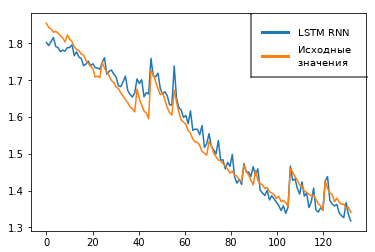
\includegraphics[width=0.5\textwidth]{pic/model.png}
  \label{fig:3}
\end{figure}
  \end{block}
\end{frame}
\begin{frame}
  \begin{block}{Исходный код:}
    \href{https://github.com/lysa0/coursework}{https://github.com/lysa0/coursework}
  \end{block}
\end{frame}
\section*{}
\begin{frame}
  \titlepage
\end{frame}
\end{document}